\chapter{Proof-of-concept implementatie met OpenMetadata}
\label{ch:poc-implementatie}

\section{Doel en positionering van de proof-of-concept}

Zoals beschreven in Hoofdstuk~\ref{ch:contextanalyse} ontstaat de grootste zichtbaarheidskloof in de huidige lineageketen bij VLAIO tussen de platinum-datasets in de Databricks-lakehouse omgeving en de daarop gebaseerde Power BI-rapporten. Deze proof-of-concept (PoC) heeft als doel om die laatste stap expliciet te maken in OpenMetadata, door Power BI-metadata systematisch te koppelen aan bestaande tabellen in de vorm van OpenMetadata-entiteiten en daaruit een bruikbare lineageketen op te bouwen voor representatieve impactanalysecases, in het bijzonder rapporten gebaseerd op de Steunster- en Krissteunster-schema’s. Dit zijn datasetmodellen in de vorm van een sterschema, die een overzicht geven van alle steun die een onderneming bij VLAIO vraagt, krijgt en geweigerd wordt, met daarbij relevante informatie over maatregelen en dossierkenmerken. Krissteunster is daarbij een uitbreiding van Steunster.\\

Hoewel de evaluatie en de illustratieve voorbeelden in dit hoofdstuk voornamelijk focussen op de Steunster/Krissteunster-rapporten, is de onderliggende aanpak bewust generiek opgezet. De naamgebaseerde mappingscripts zijn ontwikkeld voor de volledige set Power BI-datasets uit de export (momenteel 418 datasets) en leveren voor een aanzienlijk deel daarvan overeenkomsten met platinum-datasets. De proof-of-concept werd aanvankelijk getest op een beperkte subset van Steunster en Krissteunster-rapporten, maar de uitgewerkte mapping- en lineage-logica is in principe toepasbaar op alle Power BI-rapporten waarvoor een betrouwbare koppeling naar platinum-datasets beschikbaar is. De volledige end-to-end-flow, inclusief dashboardcreatie en het effectief aanmaken van lineage-edges, werd binnen deze bachelorproef bewust niet voor alle beschikbare Power BI-data uitgevoerd. Aangezien het hoofddoel van het stagebedrijf een schaalbare methode voor het gehele datalandschap was, volstond het om de werking van de PoC aan te tonen. Een volledige uitrol voor alle resterende rapporten was voor dit onderzoek dan ook niet nodig.\\

De PoC is uitgewerkt als een reeks herbruikbare Pythonscripts en Jupyter-notebooks in een Git-repository. De kernfunctionaliteit bestaat uit:
\begin{itemize}
	\item het opzetten en testen van een verbinding met de OpenMetadata-client
	\item het inlezen en verwerken van metadata over Power BI-datasets en -rapporten, en van een overzicht van platinum-datasets
	\item het genereren van mappings tussen Power BI-datasetnamen en onderliggende platinum-datasets op basis van een hulpscript
	\item het aanmaken van dashboard-entiteiten in OpenMetadata voor Power BI-rap\-por\-ten
	\item het leggen van lineage-edges tussen platinum-tabellen en de aangemaakte dashboard-entiteiten
\end{itemize}

Alle implementatiestappen zijn opgezet met het oog op herbruikbaarheid voor andere datasets dan Steunster. Lokale configuratie (JWT-token, pad naar metadatafiles) wordt daarom gescheiden gehouden van de generieke logica voor mapping en lineage-opbouw.\\

\section{Technische omgeving en architectuur}

De PoC maakt gebruik van de bestaande OpenMetadata-omgeving binnen VLAIO. De verbinding gebeurt via de publieke API-endpoint \texttt{https://omd.data-services-dev.vlaio.be/api}, met een JWT-token dat lokaal als omgevingsvariabele wordt ingelezen. Op basis daarvan wordt in het script \texttt{client\_config.py} een Open\-Me\-ta\-da\-ta-client opgebouwd, die in de rest van de repository wordt hergebruikt om entiteiten op te vragen en te creëren. Deze client is een Python SDK client, die ervoor zorgt dat je makkelijk kan interageren met de API van OpenMetadata zonder dat je zelf rechtstreekse HTTP-verzoeken moet gebruiken. De standaardservice voor Power BI-gerelateerde entiteiten is \texttt{VLAIO\_POWERBI\_TEST}. Deze service was reeds aangemaakt in OpenMetadata en indien dit niet het geval zou zijn, kan de service eenvoudig worden aangemaakt via de OpenMetadata-gebruikersinterface of via de Python-SDK.\\

De repository bevat daarnaast een aantal scripts die tijdens de ontwikkeling gebruikt werden om de interactie met de OpenMetadata-API stapsgewijs te verkennen en te valideren. Deze scripts vormen geen onderdeel van de uiteindelijke end-to-end-flow, maar hebben een belangrijke rol gespeeld in het opbouwen en testen van de kernfunctionaliteit:
\begin{itemize}
	\item \texttt{client\_config.py}: hulpfunctie om de OpenMetadata-client in te stellen en de verbinding te testen
	\item \texttt{create\_dashboard.py}: voorbeeldscript dat laat zien hoe een dashboard-entiteit aangemaakt kan worden via de SDK
	\item \texttt{add\_lineage\_edge.py}: voorbeeldscript om een lineage-edge tussen twee bestaande entiteiten toe te voegen
	\item \texttt{get\_table\_by\_id.py}: script om een tabel op te zoeken op basis van id of fully-qualified name (FQN) en het resultaat van de API-call te inspecteren
\end{itemize}

Hoewel OpenMetadata standaard een Power BI-connector aanbiedt voor het automatisch aanmaken van dashboards en lineage,\footnote{Zie de officiële documentatie van OpenMetadata voor de Power BI-connector: \url{https://docs.open-metadata.org/v1.12.x/connectors/dashboard/powerbi}.} kon deze in de VLAIO-context niet gebruikt worden. De nodige rechten en rechtstreekse toegang tot de Power BI REST API ontbreken op het niveau waarop OpenMetadata draait, waardoor een directe connectorconfiguratie niet haalbaar was. In theorie zou lineage ook volledig manueel kunnen worden opgebouwd via de gebruikersinterface, maar voor het aantal datasets en rapporten in scope zou dit een zeer arbeidsintensieve en foutgevoelige werkwijze zijn. Om die redenen is in deze PoC gekozen voor een alternatieve aanpak, waarbij Power BI-metadata uit Databricks — die daar beschikbaar is als resultaat van Power BI REST-exports — via CSV-bestanden wordt ingelezen en vervolgens via de OpenMetadata-SDK programmatisch wordt omgezet naar dashboard-entiteiten en lineage-edges.\\

Voor de end-to-end-flow rond de Steunster-case wordt gewerkt met notebooks, in het bijzonder \texttt{openmetadata\_lineage\_from\_yaml.ipynb}, waarin de volledige keten van gegevensinlees, mapping, dashboardcreatie en lineage-opbouw doorlopen wordt. Een aparte notebook (\texttt{cleanup\_steunster\_lineage\_dashboards.ipynb}) ondersteunt het opschonen van testdashboards en test-lineage, zodat de omgeving proper gehouden kan worden tijdens het ontwikkelen en testen.\\

Tokens en andere geheimen worden niet in de notebooks zelf opgeslagen, maar via een lokale \texttt{.env}-configuratie ingelezen, zodat de code zelf herbruikbaar blijft zonder gevoelige informatie prijs te geven.\\

\section{Datasets en metadata-bronnen}

De PoC combineert drie soorten metadata-bronnen:

\begin{itemize}
	\item Power BI-metadata in Databricks (tabellen met informatie over datasets en rapporten, gevoed via de Power BI REST API)
	\item een export van platinum-datasets uit de Databricks-lakehouseomgeving
	\item bestaande metadata in OpenMetadata voor Databricks-tabellen en Power BI-dashboards
\end{itemize}

De Power BI-kant wordt in deze PoC gerepresenteerd via CSV-bestanden die uit Databricks werden geëxporteerd:
\begin{itemize}
	\item \texttt{PowerBI\_Datasets.csv}: een lijst van Power BI-datasets met onder meer namen en ids;
	\item \texttt{PowerBI\_Steunster\_Datasets.csv}: één van de subsets van Power BI-datasets gebruikt voor het testen
\end{itemize}

Aan Databricks-zijde wordt gewerkt met:
\begin{itemize}
	\item \texttt{All\_Platinum\_Datasets.csv}: een overzicht van alle platinum-datasets aanwezig in de databricks omgeving
\end{itemize}

De bedoeling is dus om alle PowerBI datastes te kopellen aan de bijhorende platinum datasets. Als deze mapping vastligt kan nadien correcte lineage toegevoegd worden.  Hoewel in deze PoC gewerkt wordt met CSV-exports uit Databricks, is de gebruikte logica niet inherent afhankelijk van CSV-bestanden: in principe kan dezelfde mapping- en lineage-aanmaak ook rechtstreeks op de Databricks-tabellen worden toegepast, door de benodigde metadata direct uit de lakehouseomgeving lezen. In het kader van deze bachelorproef is gekozen voor CSV-exports als pragmatische oplossing binnen de beschikbare tijd en rechten.\\

Binnen OpenMetadata zelf zijn de Databricks-tabellen reeds geregistreerd via bestaande ingestietaken. De PoC voegt hieraan een extra laag toe. Power BI-dashboards en lineage-edges die laten zien welke platinum-tabellen de belangrijkste bron vormen voor een bepaald rapport. Om de lineage-grafieken overzichtelijk en functioneel te houden, wordt bij datasets die een sterschema volgen, specifiek gekozen voor de fact tabel(len), aangezien deze het centrum van een schema vormen met daarin de belangrijke info, terwijl dimensietabellen enkel context bieden. Bij overige datasets wordt op dezelfde manier gefocust op de voornaamste brontabel(len). Een alternatief was om een rapport-entiteit met alle tabellen van de bijhorende dataset te verbinden, maar dit zou zorgen veel meer verbindingen, waardoor de voorstelling van de lineage voor de gebruikers zeer onoverzichtelijke zou worden.

\paragraph{Afleiding van Power BI-rapporten uit Databricks.}

Omdat OpenMetadata in de huidige VLAIO-omgeving niet rechtstreeks kan verbinden met de Power BI REST API, werd gebruikgemaakt van de afgeleide Power BI-metadata die reeds onder vele tabellen in Databricks beschikbaar is (onder meer \texttt{powerbirestapi\_report} en \texttt{powerbirestapi\_dataset}). Deze tabellen waren niet vooraf gedocumenteerd voor het doel van lineage, waardoor eerst manueel onderzocht moest worden welke combinaties van kolommen en joins nodig waren om een bruikbaar overzicht van rapporten en bijbehorende datasets op te bouwen. Na het verkennen van de relevante tabellen werd onderstaande query opgesteld als basis om de Steunster-rapporten te extraheren:

\begin{lstlisting}[language=SQL, caption={Query om Power BI-rapporten en -datasets te selecteren uit Databricks}, label={lst:powerbirest-query}]
	SELECT
		r.RapportNaam,
		r.WebUrl,
		-- r.RapportOmschrijving,
		d.DatasetNaam,
		r.RapportID,
		r.DatasetID
	FROM ccdata_dev.silver.powerbirestapi_report r
	JOIN ccdata_dev.silver.powerbirestapi_dataset d
	ON r.DatasetID = d.DatasetID
	WHERE d.DatasetNaam = 'VLAIO Steunster'
	ORDER BY r.RapportNaam
	LIMIT 20;
\end{lstlisting}

De kolom \texttt{RapportOmschrijving} werd hier bewust niet gebruikt, omdat deze in de praktijk vrijwel altijd leeg bleek en dus weinig meerwaarde had voor de PoC. Indien deze ingevuld is kan je deze ook meegeven aan OpenMetadata. Op basis van de queryresultaten werd een CSV-export gemaakt die vervolgens in de notebook werd ingelezen als input voor de mapping- en lineage-scripts. Dit was noodzakelijk omdat op het moment van de implementatie nog geen permissies beschikbaar waren om vanuit Databricks rechtstreeks met de OpenMetadata-API te verbinden. Conceptueel is de aanpak echter niet beperkt tot CSV-bestanden: dezelfde SQL-query kan in een latere fase rechtstreeks als bron dienen voor een geautomatiseerde lineageflow, waarbij de resultaten zonder tussenstap naar OpenMetadata worden geschreven.\\

In de query hierboven wordt gefilterd op \texttt{DatasetNaam = 'VLAIO Steunster'} om de eerste experimenten te focussen op één concrete dataset. Deze filter is niet strikt noodzakelijk: in principe kan hetzelfde patroon zonder deze voorwaarde worden toegepast op alle rapporten in de powerbirestapi-tabellen, waarna de generieke mappinglogica de koppeling naar de onderliggende platinum-datasets voor het volledige Power BI-landschap kan maken.\\

\section{Mapping van Power BI-datasets naar platinum-datasets}

\subsection{Algemene mappingstrategie}

De kern van de PoC is een generieke mappinglaag die Power BI-datasetnamen koppelt aan de onderliggende platinum-datasets. Deze mapping gebeurt niet via handmatig ingevulde lijsten, maar via een set heuristieken die de namen in beide domeinen op verschillende manieren met elkaar vergelijkt. De implementatie is opgesplitst in twee scripts:
\begin{itemize}
	\item \texttt{\_build\_mapping.py}: bouwt een basis-mapping tussen de volledige lijst van Power BI-datasets en de platinum-datasetlijst
	\item \texttt{\_build\_mapping\_strict.py}: verfijnt de mapping en filtert op de meest betrouwbare matches
\end{itemize}

De scripts voeren eerst een normalisatie van namen uit (bijvoorbeeld lowercasing, verwijderen van speciale tekens, hanteren van consistentie bij camelCase en enkele uitzonderingen en passen vervolgens verschillende heuristieken toe om mogelijke matches te scoren.\\

In de context van deze bachelorproef wordt de mappinggenerator vooral gebruikt als hulpmiddel om een eerste, zo volledig mogelijke basisversie van de YAML configuratie voor Power BI–platinum-mapping op te bouwen en om manuele mappingarbeid te beperken. Het is niet de bedoeling dat deze scripts één-op-één als verplicht onderdeel van de toekomstige operationele processen bij VLAIO worden overgenomen, maar eerder dat ze aantonen hoe een naamgebaseerde aanpak kan helpen om een correct startpunt voor verdere verbetering te creëren.\\

\subsection{Heuristieken en outputstructuur}

De mappinglogica combineert verschillende naamgebaseerde vergelijkingsstrategieën, zoals exacte matching, deelstringvergelijkingen, fuzzy matching en token-gebaseerde vergelijkingen. Op basis van de gecombineerde scores worden potentiële koppelingen tussen Power BI- en platinum-datasets automatisch geclassificeerd naar betrouwbaarheid. De resultaten worden vervolgens weggeschreven naar aparte CSV-bestanden, zodat duidelijke matches rechtstreeks gebruikt kunnen worden en twijfelgevallen apart beschikbaar blijven voor eventuele manuele controle.\\

De mapping-output ondersteunt ook multi-mapping. Elke Power BI-dataset kan, indien nodig, aan meerdere platinum-datasets gekoppeld worden. De kolom \texttt{platinum\_datasets} bevat dan een lijst van kandidaten, en \texttt{match\_count} geeft het aantal matches aan. Dergelijke composite-situaties krijgen een aparte status, \texttt{confirmed\_multi}, zodat downstream-logica hiermee rekening kan houden. Een voorbeeld hiervan is \texttt{Krissteunster-Steunster Composite model} die gemapt moet worden naar zowel Steunster als Krissteunster.\\

In de meest recente run verwerkte de mappinggenerator 418 Power BI-datasets, waarvan 117 als \texttt{confirmed} en 4 als \texttt{confirmed\_multi} werden geclassificeerd. De overige 297 datasets bleven \texttt{unmatched}. Dat is niet noodzakelijk een tekortkoming van de mappinglogica: veel Power BI-datasets hebben geen directe of zinvolle tegenhanger in de platinum-laag en kunnen daarom normaal gezien niet gekoppeld worden. Deze niet-gematchte gevallen vragen wel een manuele controle om te onderscheiden tussen terecht niet-koppelbare datasets en uitzonderingen waarvoor de heuristieken nog verfijnd kunnen worden.\\

\paragraph{Voorbeeld van mapping-output (CSV).}

Onderstaand fragment illustreert hoe de output van het mappingscript eruitziet in \texttt{PowerBI\_to\_Platinum\_mapping\_confirmed.csv}. Hieruit blijkt dat de naam van een Power BI-dataset niet noodzakelijk exact hoeft overeen te komen met de naam van de bijhorende platinum-dataset om toch tot een correcte koppeling te komen. De gegenereerde mapping dient daarbij vooral als een eerste, reproduceerbare basis die manueel werk vermindert. Vooraleer deze mappings worden omgezet naar de YAML-configuratie die effectief gebruikt wordt voor het aanmaken van lineage, moeten ze uiteraard manueel nagekeken worden.

\begin{table}[h]
	\centering
	\small
	\begingroup
	\renewcommand{\arraystretch}{2}
	\begin{tabularx}{\textwidth}{>{\raggedright\arraybackslash}X
			>{\raggedright\arraybackslash}X
			>{\centering\arraybackslash}p{1.4cm}
			>{\centering\arraybackslash}p{1.8cm}
			>{\raggedright\arraybackslash}p{2.6cm}}
		\hline
		\textbf{Power BI-dataset} & \textbf{Platinum-dataset(s)} & \textbf{Aantal} & \textbf{Score} & \textbf{Status} \\
		\hline
		Bedrijventerreinenster & bedrijventerreinenster & 1 & 1.000 & confirmed \\
		Contactenster & contactenster & 1 & 1.000 & confirmed \\
		KRISsteunster & krissteunster & 1 & 1.000 & confirmed \\
		Krissteunster--Steunster Composite model & krissteunster;steunster & 2 & 0.990 & confirmed\_multi \\
		Corona -- Heropstartlening & r\_coronaheropstartlening & 1 & 0.980 & confirmed \\
		\hline
	\end{tabularx}
	\endgroup
	\caption{Verkort fragment uit \texttt{PowerBI\_to\_Platinum\_mapping\_confirmed.csv}.}
	\label{tab:mapping-confirmed}
\end{table}

\paragraph{Voorbeeld van Power BI-datasetmappings (YAML).}

Dat laatste is bijvoorbeeld het geval in het onderstaande fragment voor \texttt{Epplus betalingen}. Deze Power BI-dataset wordt enerzijds nog steeds logisch gekoppeld aan de platinum-dataset \texttt{r\_epplus}, maar anderzijds wordt ook expliciet de tabel \texttt{epp\_betalingen} meegegeven. Hierdoor verwijst de lineage in dit geval niet naar alle fact- of brontabellen binnen \texttt{r\_epplus}, maar enkel naar de concrete tabel waarvoor voldoende zekerheid bestaat dat ze effectief in het rapport gebruikt wordt. De YAML-structuur laat dus zowel generieke mappings op datasetniveau als meer precieze mappings op tabelniveau toe, afhankelijk van de hoeveelheid beschikbare metadata.

\begin{lstlisting}[language=YAML, caption={Fragment uit PowerBI_Dataset_Mappings.yml}, label={lst:yaml-pbi}]
	- PBIDataset: VLAIO Steunster
	  target_datasets:
		- steunster
	
	- PBIDataset: KRISsteunster
	  target_datasets:
		- krissteunster
	
	- PBIDataset: Krissteunster-Steunster Composite model
	  target_datasets:
		- krissteunster
		- steunster
	
	- PBIDataset: Dataset PBIDatasetsMetRollen
	  target_datasets:
		- r_pbidatasetsmetrollen
		
	- PBIDataset: Epplus betalingen
	  target_datasets:
		- r_epplus
	  target_tables:
		- lz02-d-dbw-ccdata-main.platinum_dev.r_epplus.epp_betalingen
	
\end{lstlisting}

\paragraph{Voorbeeld van platinum-datasetmappings (YAML).}

Aangezien lineage in OpenMetadata volgens de gangbare aanpak op tabelniveau wordt vastgelegd, volstaat het niet om enkel een koppeling te maken tussen een Power BI-dataset en een logische platinum-dataset. Daarom werd aanvullend een manuele mapping opgesteld waarin per platinum-dataset wordt vastgelegd welke concrete tabellen als meest relevante bron voor de lineage beschouwd worden. Zoals eerder vermeld wordt daarbij in de eerste plaats gekozen voor facttabellen wanneer die beschikbaar zijn, en anders voor de belangrijkste tabellen binnen de betrokken dataset.\\

In \texttt{Platinum\_Dataset\_Mappings.yml} worden de logische platinum-datasets verder vertaald naar één of meerdere technische tabel-FQN’s in Databricks. Daarbij wordt bewust met fully qualified names (FQN’s) gewerkt, omdat deze niet alleen eenduidig verwijzen naar de juiste tabel binnen de Databricks-omgeving, maar ook noodzakelijk zijn om de overeenkomstige tabelentiteiten correct op te zoeken en te gebruiken in OpenMetadata. Deze YAML-configuratie is makkelijk uitbreidbaar en aanpasbaar. Nieuwe datasets of bijkomende tabellen kunnen zonder aanpassing van de onderliggende scriptlogica worden toegevoegd, terwijl bestaande mappings ook eenvoudig verfijnd kunnen worden wanneer extra domeinkennis beschikbaar komt of de datamodellen wijzigen.

\begin{lstlisting}[language=YAML, caption={Fragment uit Platinum_Dataset_Mappings.yml}, label={lst:yaml-platinum}]
	- dataset: krissteunster
	  target_tables:
		- lz02-d-dbw-ccdata-main.platinum_dev.krissteunster.f_steun
		- lz02-d-dbw-ccdata-main.platinum_dev.krissteunster.f_steunster
		- lz02-d-dbw-ccdata-main.platinum_dev.krissteunster.f_steunster_toegevoegdewaarde
	
	- dataset: steunster
	  target_tables:
		- lz02-d-dbw-ccdata-main.platinum_dev.steunster.f_steun
\end{lstlisting}

\section{Dashboards en lineage in OpenMetadata}

\subsection{End-to-end-flow voor Steunster}

De end-to-end-aanpak voor de Steunster-rapporten bestaat uit meerdere opeenvolgende stappen. Niet al deze stappen worden in de notebook \texttt{steunster\_openmetadata\_lineage\_from\_yaml.ipynb} zelf uitgevoerd. De voorbereiding gebeurt deels vooraf en omvat het verzamelen van de nodige Power BI-metadata, het genereren en manueel valideren van de mappings, en het opstellen van de YAML-configuraties. De notebook gebruikt deze voorbereide input vervolgens om de effectieve OpenMetadata-flow uit te voeren, namelijk het opzoeken van de juiste tabel-entiteiten, het aanmaken van dashboard-entiteiten en het leggen van de overeenkomstige lineage-relaties. De volledige flow bestaat uit:
\begin{enumerate}
	\item verzamelen en voorbereiden van de nodige Power BI-metadata;
	\item bepalen welke Power BI-dataset aan elk geselecteerd rapport gekoppeld is;
	\item genereren en valideren van mappings tussen Power BI-datasets en platinum-datasets;
	\item vastleggen van de relevante platinum-tabellen in YAML-configuratie;
	\item opzoeken van de corresponderende tabel-entiteiten in OpenMetadata via hun fully qualified name of id;
	\item aanmaken van dashboard-entiteiten in OpenMetadata voor de relevante Power BI-rapporten;
	\item aanmaken van lineage-edges van de geselecteerde platinum-tabellen naar de aangemaakte dashboards.
\end{enumerate}

De focus ligt op lineage op tabelniveau: voor elk rapport wordt minstens één lineage-edge gelegd vanaf de belangrijkste platinum-tabel naar het dashboard, aangevuld met extra edges bij samengestelde datasets. Op die manier ontstaat er een visueel traceerbare keten van bronsystemen via medallion-lagen (bronze, silver, platinum) tot en met de rapportages.\\

\subsection{Belangrijkste notebook-code}

Onderstaande fragmenten tonen de kernlogica uit de notebook: het opzetten van de OpenMetadata-connectie, het inlezen van rapporten en YAML-mappings en het aanmaken van dashboards en lineage-edges. Enkel de belangrijkste code wordt weergegeven; imports, debug-prints, uitvoercontroles en enkele helperfuncties zijn weggelaten voor de leesbaarheid.

\paragraph{OpenMetadata-connectie}

Dit codefragment initialiseert de verbinding met OpenMetadata en zorgt ervoor dat de notebook geauthenticeerd kan communiceren met het metadata-platform. Eerst wordt een JWT-token uit de omgevingsvariabelen geladen, waarna de connectieparameters voor de OpenMetadata-server en de dashboardservice worden ingesteld. Tot slot wordt gecontroleerd of de verbinding succesvol tot stand komt, zodat de volgende stappen enkel worden uitgevoerd wanneer de metadata-omgeving bereikbaar is.\\

\begin{lstlisting}[language=python, caption={OpenMetadata clientconnectie}, label={lst:om-connectie}]
# (hier worden alle imports en omgevingsvariabelen geladen)
jwt = os.getenv("JWT")

# Hier wordt de OpenMetadata-host en de dashboardservice ingesteld
OM_HOST = "https://omd.data-services-dev.vlaio.be/api"
DASHBOARD_SERVICE = "VLAIO_POWERBI_TEST"

# Serverconfiguratie voor de OpenMetadata-client en eronder de SDK-client
server_config = OpenMetadataConnection(
	hostPort=OM_HOST,
	authProvider="openmetadata",
	securityConfig=OpenMetadataJWTClientConfig(jwtToken=jwt),)

# initialisatie ometa-client en SDK-client
metadata = OpenMetadata(server_config)
configure(host=OM_HOST, jwt_token=jwt)
\end{lstlisting}

\paragraph{Inlezen van rapporten en YAML-mappings}

In volgend codefragment worden enerzijds de Power BI-rapporten uit een CSV-bestand ingelezen en anderzijds de mappingbestanden in YAML-formaat verwerkt. Vervolgens worden hulpfuncties gedefinieerd om sleutels te normaliseren, lijsten van tabellen op te bouwen en dubbele waarden te verwijderen met behoud van volgorde. Op basis daarvan wordt een resolver opgebouwd die per Power BI-dataset de juiste brontabellen bepaalt, met prioriteit voor rechtstreeks opgegeven tabellen en een fallback via gekoppelde platinum-datasets. Het inladen van de Power BI-data, de mappings en de hulpfuncties zijn hier weggelaten.\\

\begin{lstlisting}[language=python, caption={PBI-data en mappings inladen en verwerken}, label={lst:yaml-logica}]
POWERBI_MAPPING_PATH = "PowerBI_Dataset_Mappings.yml"
PLATINUM_MAPPING_PATH = "Platinum_Dataset_Mappings.yml"

# Hier worden twee dictionaries aangemaakt: 
# 1) Power BI naar platinumdataset
power_bi_map = {}
for item in power_bi_yaml.get("datasets", []):
	pbi_name = str(item.get("PBIDataset", "")).strip()
	if not pbi_name:
		continue
	power_bi_map[normalize_key(pbi_name)] = {
		"target_tables": to_str_list(item.get("target_tables", [])),
		"target_datasets": to_str_list(item.get("target_datasets", [])),}

# 2) platinumdataset naar correcte tabel(len)
platinum_map = {}
for item in platinum_yaml.get("datasets", []):
	dataset_name = str(item.get("dataset", "")).strip()
	if not dataset_name:
		continue
	platinum_map[normalize_key(dataset_name)] = to_str_list(item.get("target_tables", []))
\end{lstlisting}

Na het opbouwen van de opzoektabellen wordt de logica gedefinieerd om de effectieve technische brontabellen te bepalen. De functie \texttt{resolve\_source\_table\_fqns} gebruikt hierbij een prioriteitsregeling: er wordt eerst gezocht naar direct gedefinieerde tabellen in de mapping, en bij afwezigheid daarvan wordt de koppeling gelegd via de overkoepelende platinum-datasets. Dit is zo geïmplementeerd voor de uitzonderlijke gevallen waarin wel meegegeven wordt welke specifieke tabel uit het schema gebruikt wordt. Meestal ontbreekt deze informatie en wordt gemapt naar de belangrijkste tabel(len). Tot slot wordt een hulpfunctie geïmplementeerd die de OpenMetadata-SDK aanroept om de effectieve tabelentiteiten op te zoeken op basis van hun Fully Qualified Name, die is opgebouwd als \texttt{databaseservice.database.schema.table}.\\

\begin{lstlisting}[language=python, caption={Functies voor het opzoeken van de brontabel}, label={lst:table-resolver}]
# Bepaal de bron-tabellen voor een Power BI-dataset met volgende prioriteit:
# 1. direct opgegeven target_tables in de Power BI-YAML
# 2. target_datasets uit de Power BI-YAML, vertaald via de Platinum-YAML
def resolve_source_table_fqns(dataset_name: str) -> list[str]:
	mapping = power_bi_map.get(normalize_key(dataset_name))
	if not mapping:
		return []
	
# Gebruik directe target_tables wanneer deze expliciet aanwezig zijn.
	direct_tables = mapping.get("target_tables", [])
	if direct_tables:
		return unique_preserve_order(direct_tables)
	
# Gebruik anders target_datasets en vertaal die naar tabel-FQNs.
	resolved = []
	for target_dataset in mapping.get("target_datasets", []):
		resolved.extend(platinum_map.get(normalize_key(target_dataset), []))
	return unique_preserve_order(resolved)

# Functie om een tabel op te halen via de fully-qualified name
def get_table_by_fqn(fqn: str):
	try:
		return Tables.retrieve_by_name(fqn)
	except Exception:
		return None
\end{lstlisting}

\paragraph{Aanmaken van dashboards\-en\-ti\-tei\-ten}

Vervolgens worden de ingelezen Power BI-rapporten omgezet naar dashboard-entiteiten in OpenMetadata. Daarbij wordt eerst gecontroleerd of een dashboard reeds bestaat op basis van het rapport-ID of de URL, zodat dubbele creatie vermeden wordt. Indien nog geen overeenkomstig dashboard aanwezig is, wordt een nieuwe dashboard-entiteit aangemaakt en worden de relevante identificatoren en resultaten bijgehouden voor verdere verwerking. Het is mogelijk dat verschillende rapporten verwijzen naar dezelfde Power BI-URL, dus de optie \texttt{CREATE\_IF\_WEB\_URL\_NOT\_EXISTS} staat idealiter op \texttt{False}. Hierdoor wordt voor elk rapport met een uniek id een dashboard gemaakt.\\

In onderstaande code worden de bestaande dashboards op OpenMetadata opgehaald en bijgehouden op URL en id. Deze worden later gebruikt om na te kijken of al dan niet een dashboard is aangemaakt voor een rapport, om dubbels te voorkomen.

\begin{lstlisting}[language=python, caption={Opzoeken bestaande dashboards}, label={lst:dashboards-indexeren}]
# Bepaal hoe bestaande dashboards gedetecteerd worden:
# False = controle op basis van RapportID
# True = controle op basis van WebUrl
CREATE_IF_WEB_URL_NOT_EXISTS = False

# (Hier staan enkele hulpfuncties)

# Indexeer bestaande dashboards om duplicaten te vermijden.
existing_by_url = {}
existing_by_report_id = {}

for dashboard in Dashboards.list_all():
	dashboard_url = normalize_url(to_plain_str(getattr(dashboard, "sourceUrl", "")))
	dashboard_report_id = extract_report_id(dashboard_url)

if dashboard_url and dashboard_url not in existing_by_url:
	existing_by_url[dashboard_url] = dashboard

if dashboard_report_id and dashboard_report_id not in existing_by_report_id:
	existing_by_report_id[dashboard_report_id] = dashboard
\end{lstlisting}

Vervolgens wordt er voor elk rapport uit de bronbestanden een dashboard-entiteit aangemaakt via de OpenMetadata-SDK. Het is belangrijk hierbij op te merken dat deze entiteit in OpenMetadata dient als een metadatarepresentatie of een proxy en niet het werkelijke dashboard bevat. De entiteit krijgt standaard de naam van het bijbehorende Power BI-rapport. Door bij de creatie aanvullende parameters zoals een omschrijving en de \texttt{sourceUrl} mee te geven, wordt de traceerbaarheid vergroot en kan een gebruiker vanuit de OpenMetadata-interface direct navigeren naar het effectieve rapport in de Power BI-service. Ten slotte wordt ook een dataframe opgebouwd en weergegeven zodat zichtbaar is welke dashboards aangemaakt of overgeslagen zijn; deze code is hier weggelaten.\\

\begin{lstlisting}[language=python, caption={Dashboards maken en posten naar OpenMetadata}, label={lst:dashboards-aanmaken}]
# Alle rapporten van de Power BI REST API worden doorlopen
for _, row in df.iterrows():
	rapport_naam = str(row["RapportNaam"]).strip()
	web_url = str(row["WebUrl"]).strip()
	dataset_naam = str(row["DatasetNaam"]).strip()
	rapport_id = str(row["RapportID"]).strip()
	dataset_id = str(row["DatasetID"]).strip()

# Zoek de gekoppelde brontabellen op via de YAML-resolver
	source_fqns = resolve_source_table_fqns(dataset_naam)

	normalized_url = normalize_url(web_url)
	normalized_report_id = rapport_id.lower()
	existing_dashboard = None

# Kies de gewenste controlelogica voor reeds bestaande dashboards
	if CREATE_IF_WEB_URL_NOT_EXISTS:
		existing_dashboard = (created_by_url.get(normalized_url) or existing_by_url.get(normalized_url))
		check_mode = "WebUrl"
	else:
		existing_dashboard = (created_by_report_id.get(normalized_report_id) or existing_by_report_id.get(normalized_report_id))
	check_mode = "RapportID"

# Gebruik een bestaand dashboard wanneer dat al aanwezig is
	if existing_dashboard is not None:
		dashboard_id = existing_dashboard.id
		dashboard_fqn = to_plain_str(existing_dashboard.fullyQualifiedName)
		dashboard_status = f"existing ({check_mode} al aanwezig)"
# Maak anders een nieuwe dashboardentiteit aan
	else:
		request = CreateDashboardRequest(
			name=rapport_naam,
			displayName=rapport_naam,
			service=DASHBOARD_SERVICE,
			description=f"Dashboard aangemaakt vanuit CSV voor dataset {dataset_naam}.",
			sourceUrl=web_url,)
	
		try:
			dashboard = Dashboards.create(request)
			dashboard_id = dashboard.id
			dashboard_fqn = to_plain_str(dashboard.fullyQualifiedName)
			dashboard_status = "created"
	
			created_by_url[normalized_url] = dashboard
			if normalized_report_id:
				created_by_report_id[normalized_report_id] = dashboard
		except Exception as exc:
			dashboard_id = None
			dashboard_fqn = None
			dashboard_status = f"error: {exc}"
\end{lstlisting}

\paragraph{Aanleggen van lineage-edges}

In dit laatste codefragment worden de lineage-relaties tussen de gevonden brontabellen en de aangemaakte dashboards toegevoegd. De code doorloopt de verwerkte rapporten en voert per brontabel twee controles uit. Er wordt geverifieerd of de brontabel daadwerkelijk bestaat in OpenMetadata en deze lineage relatie nog niet is aangemaakt. Indien beide controles succesvol zijn, wordt er via een \texttt{AddLineageRequest} een expliciete koppeling aangemaakt. Listing~\ref{lst:lineage} toont deze logica, waarbij de declaraties van variabelen en logging-mechanismen zijn ingekort. De logging bouwt een dataframe met elk verwerkt rapport en daarbij zowel de status van het aanmaken van het dashboard als de lineage-edge(s). Zo kan je snel zien of alles correct verloopt.

\begin{lstlisting}[language=python, caption={Lineage aanleggen in OpenMetadata}, label={lst:lineage}]
lineage_results = []

for _, row in dashboards_df.iterrows():
	RapportNaam = row["RapportNaam"]
	DatasetNaam = row["DatasetNaam"]
	RapportID = row["RapportID"]
	# Hier worden de alle andere variabelen ingesteld die nodig zijn voor AddLineageRequest en logging
	
	if has_dashboard and source_fqns:
		for source_fqn in source_fqns:
			source_table = get_table_by_fqn(source_fqn)
			if not source_table:
				table_statuses.append(f"skipped:not_found:{source_fqn}")
				continue
	
			pair_key = f"{source_table.id}->{dashboard_id}"
			if pair_key in seen_lineage_pairs:
				table_statuses.append(f"skipped:duplicate_pair:{source_fqn}")
				continue
			try:
				req = AddLineageRequest(
					edge=EntitiesEdge(
						description=f"{DatasetNaam} voedt Power BI-rapport '{RapportNaam}'",
						fromEntity=EntityReference(id=source_table.id, type="table"),
						toEntity=EntityReference(id=dashboard_id, type="dashboard"),
						lineageDetails=LineageDetails(
							source="Manual",
							description="Automatisch toegevoegd via notebook op basis van YAML-mappings")))
				metadata.add_lineage(data=req)
				seen_lineage_pairs.add(pair_key)
				created_count += 1
				table_statuses.append(f"created:{source_fqn}")
			except Exception as exc:
				table_statuses.append(f"error:{source_fqn}:{exc}")
# (hier worden lineage_results en logging opgebouwd)
\end{lstlisting}

\subsection{Lineage voor composite-modellen}

In gevallen waar een Power BI-model meerdere platinum-datasets combineert, maakt de PoC gebruik van de \texttt{confirmed\_multi}-status. De mapping-output bevat dan meerdere platinum-datasets in de kolom \texttt{platinum\_datasets}, en de lineage-logica genereert voor elk van deze datasets een aparte edge richting hetzelfde dashboard. Hierdoor wordt zichtbaar dat een rapport afhankelijk is van meer dan één dataset in de platinum-laag, wat belangrijk is voor impactanalyses: een wijziging in één van de onderliggende datasets kan potentieel invloed hebben op het volledige rapport.\\

De Krissteunster-Steunster-case is hiervan een concreet voorbeeld. De composite Power BI-dataset wordt gekoppeld aan zowel een \texttt{krissteunster}- als een \texttt{steunster}-platinumdataset, zodat analisten in OpenMetadata onmiddellijk zien dat wijzigingen in één van beide datasets impact kunnen hebben op dezelfde rapportage.\\

\section{Beheer en opschoning van testartefacten}

Tijdens de iteratieve ontwikkeling van de PoC is het noodzakelijk om dashboards en lineage-edges regelmatig opnieuw te creëren en te verwijderen. Hiervoor wordt de notebook \texttt{cleanup\_steunster\_lineage\_dashboards.ipynb} gebruikt.\\

In deze notebook worden de aangemaakte dashboards op basis van naam of id opgezocht. Omdat naamnormalisatie soms leidt tot ambiguïteit, wordt de delete-operatie bij voorkeur uitgevoerd op basis van de unieke id die in OpenMetadata aan elk dashboard verbonden is. De notebook verwijdert vervolgens zowel de dashboard-entiteiten als de bijhorende lineage-edges, zodat er geen verouderde of dubbele relaties in de metadata achterblijven.\\

Praktisch kwamen tijdens het testen enkele terugkerende aandachtspunten naar voren:
\begin{itemize}
	\item JWT-tokens vervallen regelmatig tijdens langere sessies in de notebookomgeving. In dat geval moet de kernel herstart worden en de configuratiecel opnieuw uitgevoerd worden, zodat de client opnieuw met een geldig token kan werken.
	\item De scripts en notebooks zijn gevoelig voor bestandslocaties. Sommige flows verwachten CSV's in een \texttt{Datasets}-submap, andere in de root van de repository. In de documentatie wordt daarom expliciet vermeld welke paden voor welke notebook gebruikt worden, om reproductieproblemen te voorkomen.
\end{itemize}

\section{Beperkingen en randvoorwaarden}

De beschreven implementatie is bewust opgezet als proof-of-concept en kent een aantal belangrijke beperkingen die van invloed zijn op de interpretatie van de resultaten.\\

\subsection{Beperkingen van de naamgebaseerde mapping}

Ten eerste is de mappinglogica volledig naamgebaseerd. Hoewel de gebruikte naamgebasseerde regels in veel gevallen goede resultaten opleveren, blijft de betrouwbaarheid afhankelijk van consistente en informatieve naamgeving aan zowel Power BI- als Databricks-zijde. Datasets met zeer generieke of sterk afwijkende namen blijven \texttt{unmatched} en vallen buiten de scope van de huidige PoC. Een bijkomend gevolg van het ontbreken van een bruikbare Power BI-connector is dat de PoC voor zijn mappings volledig steunt op de Power BI-REST-API metadata in Databricks en de daaruit afgeleide data. In de huidige implementatie worden alle unieke Power BI-datasets uit deze exports opgenomen in de mapping-flow en vergeleken met de lijst van platinum-datasets. Voor de datasets die vandaag in scope zijn, levert dit in combinatie met de gebruikte naamgebasseerde regels een set mappings op die in de praktijk nagenoeg volledig correct is.\\

\subsection{Beperkingen van de naamgebaseerde mapping}

De mappinglogica werkt volledig op basis van namen, wat enkele uitdagingen met zich meebrengt. De data uit de PowerBi rest API exports in Databricks, die gebruikt wordt om de datasetnaam te achterhalen laat duidelijk zien hoe Power BI achter de schermen werkt. Namen zoals \textit{"model coosy PRD  14-01-2026"} of \textit{"Bedrijventerreinenster_0126"} zijn de titels die ontwikkelaars aan hun lokale \texttt{.pbix}-bestanden hebben gegeven vlak voordat ze deze publiceerden. Omdat mensen hun bestanden vaak handmatig datumstempels, versienummers of toevoegingen zoals 'dev' of 'Dataset' meegeven, ontstaat er een kloof met de strakke, technische tabelnamen in de platinum-laag.

Wanneer een bestand een naam krijgt die totaal niet meer lijkt op de oorspronkelijke bron, lukt het niet om het rapport te mappen. De dataset blijft dan \texttt{unmatched}. Met een puur naamgebaseerde methode is het in zulke gevallen technisch simpelweg onmogelijk om een automatische koppeling te leggen, aangezien er geen enkele tekstuele gelijkenis is om mee te vergelijken. Daarnaast is het ook belangrijk om te weten dat niet elk Power BI-rapport data gebruikt uit Databricks. Sommige rapporten zijn bijvoorbeeld gebasseerd op een lokale Excel-sheet of een SharePoint-lijst. Omdat deze bronnen niet in de platinum-laag bestaan, kunnen ze ook nooit automatisch gemapt worden.

Dit betekent dat je een naamgebaseerd systeem nooit blindelings kan gebruiken in een productie omgeving. Daar zal er altijd een manuele controle nodig blijven om de twijfelgevallen en de \texttt{unmatched}-rapporten na te kijken en eventueel handmatig toe te voegen aan de YAML. Dit is precies waarom de uiteindelijke mappings niet hardgecodeerd in het script zitten, maar worden opgeslagen in een flexibel YAML-bestand dat eenvoudig uitgebreid kan worden.

\subsection{Rol en onderhoud van de YAML-mappings}

In de huidige opzet vormen de gegenereerde YAML-mappings naast de lineage logica het belangrijkste resultaat voor VLAIO: zij leggen vast welke Power BI-datasets aan welke platinum-tabellen gekoppeld worden en worden rechtstreeks gebruikt in de end-to-end-workflows. De Python-scripts voor mapping zijn in de eerste plaats onderzoeks- en ondersteunende tools om deze YAML sneller en consistenter op te bouwen. VLAIO kan er in de toekomst voor kiezen om deze scripts al dan niet opnieuw te gebruiken, maar het is even goed mogelijk om de YAML zelf aan te passen wanneer er nieuwe datasets bijkomen of gewijzigd worden. In de meest recente versie van de YAML-workflows dekken de gegenereerde mappings vrijwel alle relevante rapporten binnen de PoC-scope. Om deze workflows in de toekomst correct te laten blijven werken, is het wel noodzakelijk dat nieuwe of aangepaste Power BI-datasets een naam krijgen die inhoudelijk aansluit bij de corresponderende platinum-dataset. Wanneer datasetnamen sterk afwijken of generiek geformuleerd zijn, neemt de kans toe dat ze niet automatisch gematcht worden en manuele aanvulling of bijsturing van de mapping nodig is.\\

\subsection{Beperkingen van lineage op kolomniveau}

Ten tweede is de lineage in deze PoC bewust beperkt tot tabelniveau. Nadat een tabel-level lineage is aangelegd op OpenMetadata is het mogelijk om de lineage uit te breiden tot op kolom-nieveau. Dit zou zorgen voor een beter inzicht, aangezien je voor een waarde in een rapport de specifieke kolom(men) zou kunnen nagaan waaruit deze is opgebouwd, alsook de onderliggende transformaties. Nadat er succesvol tabel lineage was voorzien, werd er onderzocht hoe dit uitbreidbaar is tot op kolomniveau. Dit is mogelijk op twee manieren. De eerste is opnieuw een mapping aanmaken die een bronkolom met een eindkolom verbindt. Aangezien  er op kolomniveau geen data beschikbaar is in de PowerBi REST API, zou een mapping tussen kolommen en queries per rapport manueel moeten aangemaakt en onderhouden worden, met een groot risico op fouten en verouderde mappings. De tweede manier is om te werken met de \texttt{SDL Lineage Workflow} van OpenMetadata. Hieraan kan je de \texttt{INSERT INTO ... SELECT SQl Queries} meegeven, die een PowerBi rapport voedt. Die queries worden dan automatisch geparset om de kolomrelaties te ontdekken. Tijdens een bijkomende sync-meeting met de betrokken data-engineers en BI-ontwikkelaars werd bevestigd dat kolomniveau-lineage richting Power BI-rapporten in de huidige VLAIO-context niet op een betrouwbare en onderhoudbare manier kan worden uitgewerkt. OpenMetadata toont wel de queries die in Databricks worden uitgevoerd, maar maakt niet duidelijk welk systeem of rapport een bepaalde query heeft getriggerd, zodat niet eenduidig kan worden afgeleid of een query afkomstig is van Power BI, een Databricks-gebruiker of een intern proces. Daardoor is automatische kolomlineage richting een specifiek Power BI-rapport vandaag niet haalbaar op schaal. De manuele oplossing, via Python-code die de OpenMetadata-API aanstuurt om per rapport kolomlineage in te vullen, werd in de meeting ook beoordeeld als weinig realistisch en een “maintenance hell”.\\

Om die redenen werd in overleg besloten om kolomniveau-lineage buiten de scope van deze bachelorproef te houden en te focussen op een robuuste lineage op tabelniveau, waarin zichtbaar wordt welke platinum-tabellen de belangrijkste bron vormen voor een rapport. Meer gedetailleerde of manuele verrijking kan in de toekomst eventueel case per case worden toegepast voor een beperkt aantal kritieke rapporten, maar wordt niet als algemene aanpak beschouwd.\\

\subsection{Scope van de implementatie}

Tot slot dekt de huidige end-to-endimplementatie slechts een deel van het VLAIO-rapportagelandschap. De generieke mappinggenerator wordt wel toegepast op de volledige lijst van Power BI-datasets uit de export en levert voor een aanzienlijk deel daarvan betrouwbare \texttt{confirmed}-mappings naar platinum-datasets op. In de notebooks en YAML-workflows wordt de flow van mapping naar dashboardcreatie en lineage-opbouw echter alleen volledig uitgevoerd voor een geselecteerde subset van rapporten, met de Steunster/Krissteunster-case als belangrijkste voorbeeld. De resultaten van de gebruikersevaluatie in latere hoofdstukken moeten dan ook gelezen worden als indicaties binnen deze PoC-scope, en niet als bewijs dat het volledige landschap vandaag al end-to-end in OpenMetadata is doorgetrokken.\\

\subsection{Visuele voorstelling en praktische use cases}

In deze sectie staan enkele concrete visualisaties van de lineage in OpenMetadata. De toegevoegde waarde van deze PoC uit zich in de praktijk via twee concrete scenario's: het traceren van de herkomst vanaf een specifiek rapport, en het inschatten van de impact vanaf een centrale dataset.

Ten eerste maakt het platform het mogelijk om vanuit de business-omgeving terug te redeneren naar de bron (upstream lineage). Wanneer een eindgebruiker twijfelt over de data in een specifiek dashboard, kan via de gebruikersinterface van OpenMetadata in gemakkelijk worden gecontroleerd welke platinum-dataset de basis vormt. In Figuur~\ref{fig:lineage_steun_rep} en Figuur~\ref{fig:lineage_kris_rep} is dit respectievelijk zichtbaar voor een rapport op basis van het \texttt{steunster}- en het \texttt{krissteunster}-model. Dit lost de eerder besproken 'zichtbaarheidskloof' op, aangezien de gebruiker niet langer in de Power BI-instellingen of Databricks-notebooks hoeft te zoeken naar de achterliggende databron.

\begin{figure}[htbp]
	\centering
	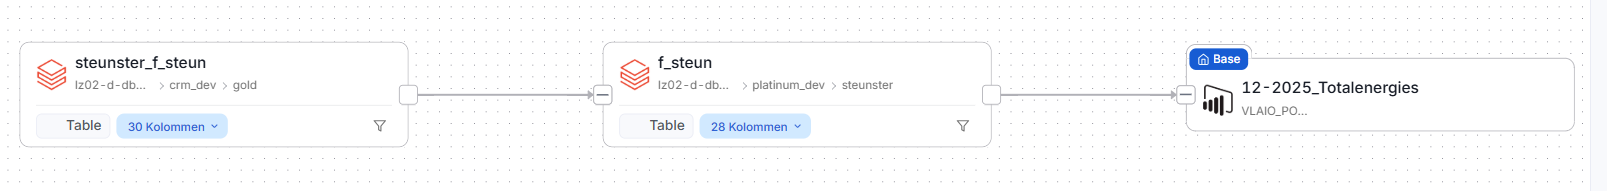
\includegraphics[width=0.9\textwidth]{images/rapport_steunster.png}
	\caption{Upstream lineage: van een specifiek Steunster Power BI-rapport terugzoeken naar de onderliggende platinum-dataset.}
	\label{fig:lineage_steun_rep}
\end{figure}

\begin{figure}[htbp]
	\centering
	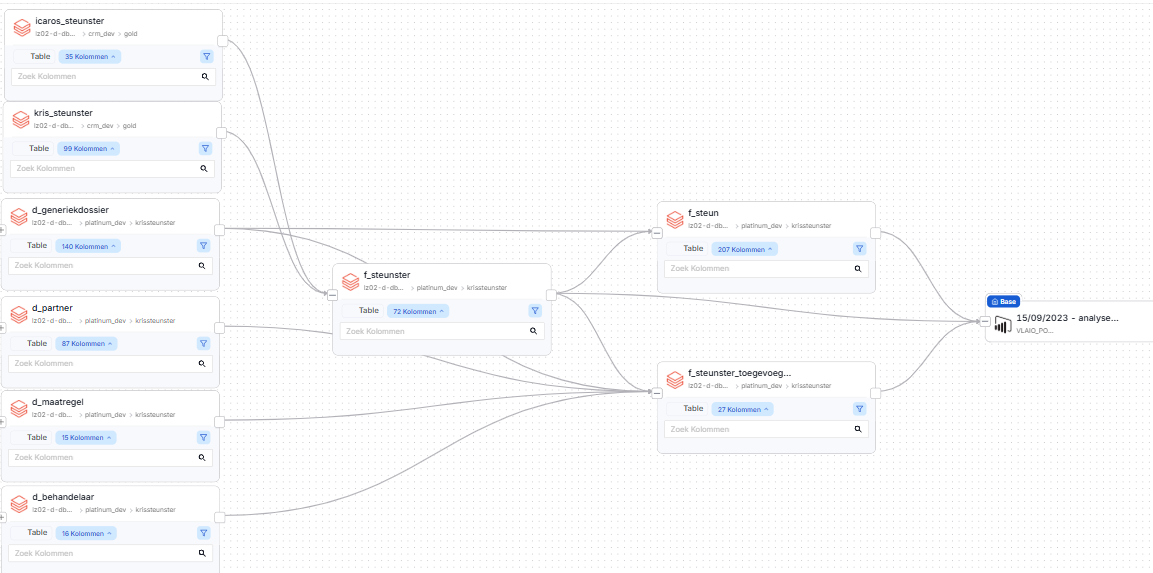
\includegraphics[width=0.9\textwidth]{images/rapport_krissteunster.png}
	\caption{Upstream lineage: van een specifiek Krissteunster Power BI-rapport terugzoeken naar de onderliggende platinum-dataset.}
	\label{fig:lineage_kris_rep}
\end{figure}

Het tweede scenario draait om impactanalyse vanuit het perspectief van databeheer (downstream lineage). Voor data-engineers of beheerders is het cruciaal om te weten wat de gevolgen zijn als een tabel in de platinum-laag of een onderliggende laag gewijzigd wordt. Figuur~\ref{fig:lineage_dataset_impact} illustreert hoe de nieuwe metadata integreert in het grotere geheel. De figuur toont niet alleen de reeds bestaande database-views, maar ook de volledige set Power BI-rapporten die via deze PoC succesvol aan de centrale \texttt{steunster}-tabel zijn gekoppeld. Mocht er in de toekomst iets veranderen aan de structuur van deze platinum-dataset of een onderliggende dataset, dan is direct duidelijk welke rapporten risico lopen en welke business-eigenaren geïnformeerd moeten worden.

\begin{figure}[htbp]
	\centering
	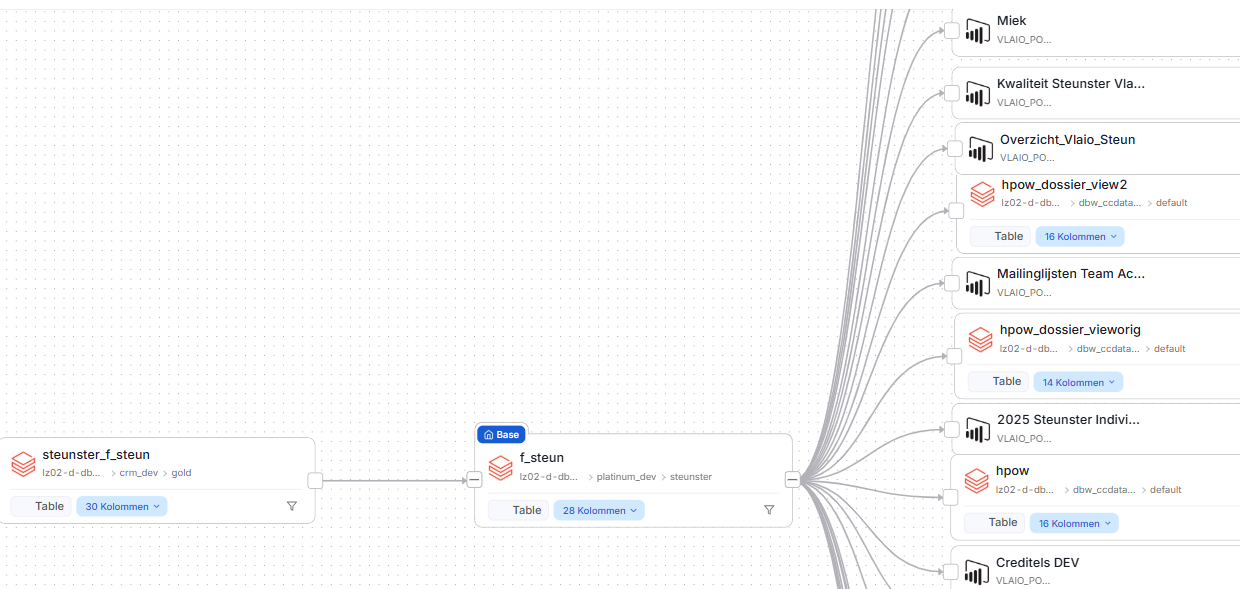
\includegraphics[width=0.9\textwidth]{images/dataset_steunster_impact.png}
	\caption{Downstream lineage: alle gekoppelde Power BI-rapporten een dataset.}
	\label{fig:lineage_dataset_impact}
\end{figure}